\section{Discussion} \label{discussion}

\textbf{Heterogeneity in single-cell data}
Because of \texttt{gamdid}'s flexible approach, it captures the heterogeneity of single-cell data that is, by design, missed by conventional DA methods. In the case study, \texttt{gamdid} identifies three features that are not detected by conventional DA methods as the distributional differences do not involve a sufficiently large mean shift.\\
More importantly, even the 52 features detected by both DA and DD methods further emphasize the need to account for heterogeneity in single-cell data. Indeed, for the majority of these features, the distributional difference extends beyond a pure mean shift. This is illustrated by \texttt{gamdid}'s visualization which reveals the important nuances of these more complex distributional patterns.\\
Four representative examples are provided in Figure \ref{fig:caseStudy_exs}. Notably, in all four examples the detected differential regions align closely with the regions of the distribution where melanoma cells were spiked in, underscoring the utility of \texttt{gamdid}'s visualization.
\\
\\
\textbf{Ranking of significant features}
Notably, the ranking of significant features is of increasing interest in proteomics, and \texttt{gamdid} offers a key advantage in this regard. For DA features, the \texttt{gamdid} ranking is very similar to that of top-performing DA methods (which is not the case for \texttt{distinct}, see Table \ref{tab:only_msqrob2}). Moreover, \texttt{gamdid} can also prioritize interesting features that are completely overlooked by DA methods. This is illustrated in Table \ref{tab:only_gamdid}, which shows that two out of the three features exclusively detected by \texttt{gamdid} are assigned high p-values by \texttt{msqrob2}.
\\
\\
\textbf{Conceptual difference between \texttt{gamdid} and \texttt{distinct}}
The simulation results reflect a fundamental difference in how \texttt{distinct} and the GAM methodology characterize distributional differences between groups. \texttt{distinct} operates on empirical cumulative distribution functions (ECDFs) and quantifies the mean difference between the ECDFs of two groups. By design, this mean ECDF difference is sensitive to sustained, global displacements of probability mass. The GAM-based approach, however, models the density function of each group. Because density estimation is inherently local, the GAM is particularly well-suited to detect distributional changes that are concentrated in specific regions of the distribution.\\
Figure \ref{fig:distinctVSgamdid}A--B illustrates this using a feature from the Petrosius DB simulations that exhibits a local change without substantially displacing the bulk of the probability mass. In this case, the mean difference between the ECDFs of the two groups remains modest, resulting in reduced power for \texttt{distinct}, whereas the GAM-based method is able to successfully identify the differential region.


Conversely, distributional changes like mean shifts produce large, sustained differences between the ECDFs of two groups and are therefore readily detected by \texttt{distinct}. The GAM-based method, however, exhibits reduced power in such settings, as mean shifts constitute diffuse, global changes that do not concentrate in any particular local region of the distribution. This behavior is illustrated in Figure \ref{fig:distinctVSgamdid}C--D, which presents a feature from the Petrosius DE simulations. This example shows an accumulated difference between the ECDFs, while the GAM method is not able to detect differential regions.\\
This motivates the aggregation of GAM-derived p-values with those from \texttt{msqrob2}, which is specifically designed to detect mean shifts with high sensitivity.

\begin{figure}[H]
    \centering
    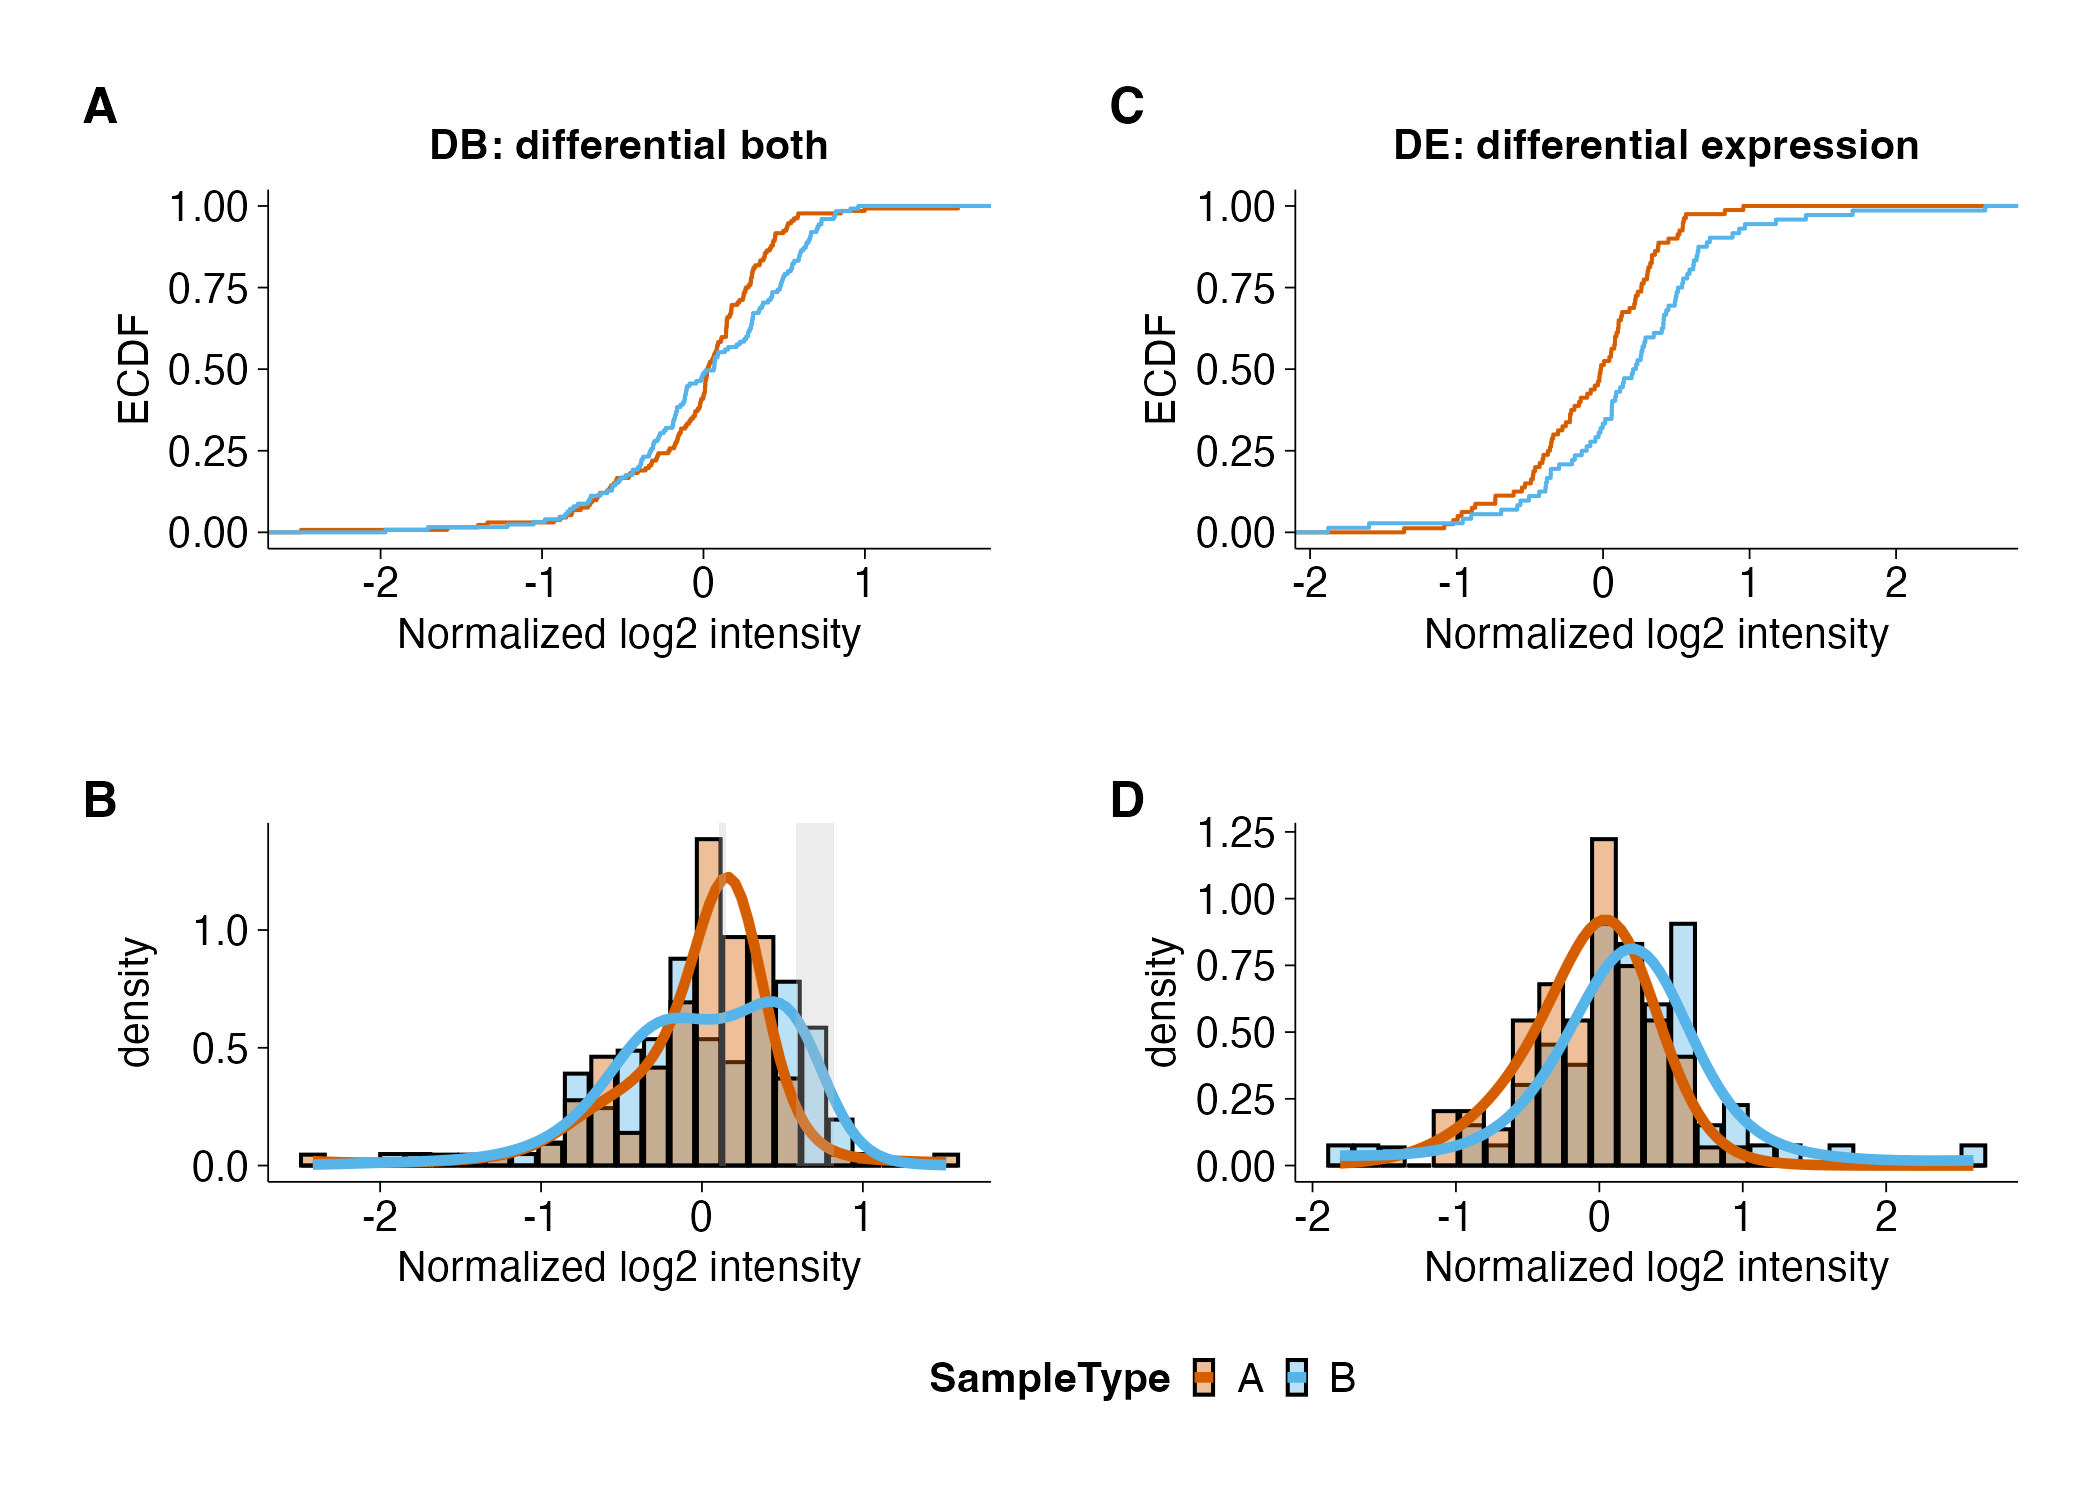
\includegraphics[width=0.85\linewidth]{figs/fig8.jpg}
    \captionsetup{labelfont={bf,small}}
    \caption{\textbf{Conceptual difference between distinct and gamdid} Comparison of how distinct (ECDF curves, top) and gamdid (density visualization, bottom) characterize two features from the Petrosius simulations. \textbf{A--B}: A feature from the DB scenario, detected by gamdid (FDR adjusted p-value = 0.012) and not by distinct (FDR adjusted p-value = 0.278). The mean ECDF difference (used by distinct) between groups is modest (A) because the induced bimodality does not produce a sustained, global displacement of probability mass, while the gamdid visualization (B) reveals the local bimodality clearly and the difference smoother identifies the specific regions where the densities diverge (gray shading). \textbf{C--D}: A feature with a pure mean shift (DE), detected by distinct (FDR adjusted p-value = 0.020) and not by the standalone GAM method before aggregation (FDR adjusted p-value = 0.227). The ECDF curves (C) show a large, sustained horizontal displacement between groups, whereas the GAM fits (D) overlap and show no identifiable differential region, reflecting the GAM's reduced power for diffuse, global distributional changes. distinct is thus more sensitive to sustained, global ECDF displacements, while the GAM's density-based, inherently local approach is better suited to detecting concentrated, shape-based differences. This complementarity motivates the aggregation of GAM p-values with msqrob2 p-values: after aggregation, the DE feature (C--D) is detected by gamdid (FDR adjusted p-value = 0.029).}
    \label{fig:distinctVSgamdid}
\end{figure}


\textbf{P-value aggregation}
The aggregated p-value in \texttt{gamdid} combines the local sensitivity of the GAM with the established power of \texttt{msqrob2} for mean-based inference, ensuring that \texttt{gamdid} is well-suited to detect any form of distributional difference. As expected, a modest loss of power relative to each individual component is observed in scenarios where only one of the two components contributes meaningfully: the DE scenario for the GAM component, and the DV and DB scenarios for \texttt{msqrob2}. This is an inherent consequence of p-value aggregation when one of the contributing p-values carries no signal. In scenarios where the distributional change involves both a mean shift and a difference in shape, however, \texttt{gamdid} combines the strength of both methods and outperforms each method separately, demonstrating the practical benefit of the aggregation strategy.
\\
\\
\textbf{FDR control}
\texttt{gamdid} achieves conservative FDR control at the nominal 5\% threshold throughout all simulations.
\\
\\
\textbf{Computational efficiency}
To evaluate computational efficiency, the runtime of both \texttt{gamdid} and \texttt{distinct} was measured on the spike-in case study dataset, comprising 1316 features and 824 cells. Each method was executed on a single core, and runtimes were averaged across ten independent runs. The mean runtime for \texttt{gamdid} was 16 seconds, whereas \texttt{distinct} required 256 seconds on average, indicating that \texttt{gamdid} achieved a speedup of more than fifteen-fold (see supplementary Figure \ref{fig:runtime}).


This can be attributed to two key factors. First, \texttt{gamdid} does not rely on permutation-based inference as \texttt{distinct} does. Second, as \texttt{distinct} cannot handle missing values, all missing observations must be removed on a per-feature basis prior to analysis.
\\
\\
\textbf{Outlook}
The development of \texttt{gamdid} represents a significant advance toward a more comprehensive interpretation of the information in single-cell proteomics data. By extending differential analysis beyond mean-based comparisons, \texttt{gamdid} enables the systematic investigation of distributional changes and thereby facilitates a more detailed characterization of cellular heterogeneity. This functionality uncovers biologically relevant variation that has remained largely unexplored by existing data analysis frameworks.\\
As single-cell proteomics technologies continue to mature and datasets grow in size and complexity, the ability to detect and interpret subtle distributional differences will become increasingly important. We therefore anticipate that \texttt{gamdid} can find applications not only in the comparison of cell types and conditions, but also in the identification of subpopulations, or the characterization of transitional cell states.\\
More broadly, the framework presented here is not intrinsically limited to proteomics and could, in principle, be adapted to other single-cell modalities, including single-cell transcriptomics, metabolomics and flow cytometry, where distributional heterogeneity likewise constitutes an important source of biological information. As such, \texttt{gamdid} has the potential to support a broader methodological shift toward distributional approaches in single-cell data analysis, enabling a more comprehensive characterization of cellular variation beyond changes in average abundance levels.


%The \texttt{msqrob2} analysis is slightly too liberal in the Leduc dataset, which is likely attributable to correlation between the proteins.


%\textbf{Leduc vs Petrosius}
%All methods exhibit reduced performance in the Petrosius simulations relative to the Leduc simulations. And interestingly, the performance gap is more pronounced, with \texttt{gamdid} substantially outperforming \texttt{distinct} on the Petrosius dataset.\\
%This difference is primarily attributable to the smaller sample size in the Petrosius dataset, which negatively impacts the permutation-based inference of \texttt{distinct}, as a limited number of permutations reduces the resolution of the resulting null distribution.\\
%To evaluate this, we subsampled the Leduc dataset such that the average number of non-missing observations per group over all feature matched that of the Petrosius dataset. The resulting FDP-TPP curves, shown in figure \ref{fig:leducsims_gamdid_subsample}, demonstrate similar trends as those observed in the Petrosius simulations. Most notably, this confirms that \texttt{gamdid} exhibits higher power than \texttt{distinct} under small-sample conditions, which has practical implications for the analysis of single-cell proteomics datasets where the number of cells per condition is limited.

%\begin{figure}[H]
%    \centering
%    \includegraphics[scale=0.2]{figs/fig17.jpg}
%    \caption{\textbf{Subsample simulation results for \texttt{gamdid}} fdp-tpp curves for \texttt{gamdid} and \texttt{distinct} for comparing two groups in the Leduc dataset under different simulations scenarios after subsampling}
%    \label{fig:leducsims_gamdid_subsample}
%\end{figure}
